
\section{B2}

\subsection{B2.1}

\subsubsection{A}

$R_{1,2} \subseteq S_1 \times S_2 =$

$\{(s_0,s'_0),(s_0,s'_3), (s_1,{s'}_1),(s_1,s'_2),(s_2,s'_1),(s_2,s'_2),(s_3,s'_1),(s_3,s'_2),$

$(s_4,s'_0),(s_4,s'_3),(s_5,s'_0),(s_5,s'_3)\}$

\subsubsection{B}

Property (1):

$(s_1,s_2) \in R \rightarrow L_1(s_1) = L_2(s_2)$

$L(s_0)=L(s'_0)=L(s'_3)=\{(\phi_1)\}$

$L(s_1)=L(s'_1)=L(s'_2)=\{(\phi_2)\}$

$L(s_2)=L(s'_1)=L(s'_2)=\{(\phi_2)\}$

$L(s_3)=L(s'_1)=L(s'_2)=\{(\phi_2)\}$

$L(s_4)=L(s'_0)=L(s'_3)=\{(\phi_1)\}$

$L(s_5)=L(s'_0)=L(s'_3)=\{(\phi_1)\}$

States have same labelling function.

\indent

\noindent
Property(2):

$\forall (s_1, s_2) \in R:$

$\forall s'_1 \in Post(s_1): \exists s'_2 \in Post(s_2): (s'_1, s'_2) \in R$

for $(s_0, s'_0):$

$s'_1 \in Post(s_0)=\{(s_1),(s_2),(s_3)\}$

$s'_2 \in Post(s'_0)=\{(s'_1),(s'_2)\}$

$\{(s_1,s'_1), (s_2,s'_2),(s_3,s'_2)\} \subseteq R.$

the same condition for the other pairs.

\indent

\noindent
Property (3):

$\forall (s_1, s_2) \in R:$

$\forall s'_2 \in Post(s_2): \exists s'_1 \in Post(s_1): (s'_1, s'_2) \in R$

for $(s_0, s'_0):$

$s'_2 \in Post(s'_0)=\{(s'_1),(s'_2)\}$

$s'_1 \in Post(s_0)=\{(s_1),(s_2),(s_3)\}$

$\{(s_1,s'_1), (s_2,s'_2)\} \subseteq R.$

the same condition for the other pairs.

\indent

\noindent
Property (I):

forall initial states $s_1$ of $M_1$ there is an initial state $s_2$ of $M_2$ with $(s_1, s_2) \in R$, and vice versa.

\indent

\noindent
as above proved that all properties are verified, this imply $M_1$ and $M_2$ are bisimulation relation. Since we have mapped all the states in $M_1$ is related to a state in $M_2$, so they are maximal.

\subsubsection{C}

$R_{1,1} \subseteq S_1 \times S_1 = $

$\{(s_0,s'_0),(s_0, s'_4),(s_0, s'_5),(s_4,s'_0),(s_4,s'_4),(s_4,s'_5),(s_5,s'_0),(s_5,s'_4),(s_5,s'_5),$

$(s_1,s'_1),(s_1,s'_2),(s_1,s'_3),(s_2,s'_1),(s_2,s'_2),(s_2,s'_3),(s_3,s'_1),(s_3,s'_2),(s_3,s'_3)\}$

\subsubsection{D}

$R_{1,1}$ is matces the verified properties,which is same as proved at above the question C.

\subsubsection{E}

Bisimulation quotient $M_1/\sim$ of $M_1$:

$S = \{s_0, s_1\}$

$I = {s_0}$

$\rightarrow = \{(s_0, s_1), (s_1, s_0)\}$

$AP = \{\Phi_1, \Phi_2\}$

$L = \{(s_0, \{\Phi_1\}), (s_1, \{\Phi_2\})\}$

Largest because all states with same labellings are related.

\subsubsection{F}

Yes, this is bisimilar to $M_2$. and the largest bisimulation relation between them are:

$(s_0,s'_0),(s_0,s'_3),(s_1,s'_1),(s_1,s'_2)$

\subsection{B2.2}

First, the formula is converted into existential normal form:

$\neg (EX \Phi_1) \wedge (\neg (EG \neg \Phi_2))$

The abstract syntax tree consists purely of state formula,
with the path operators included with their enclosing path quantifier:

\begin{figure}[!htb]
\centering
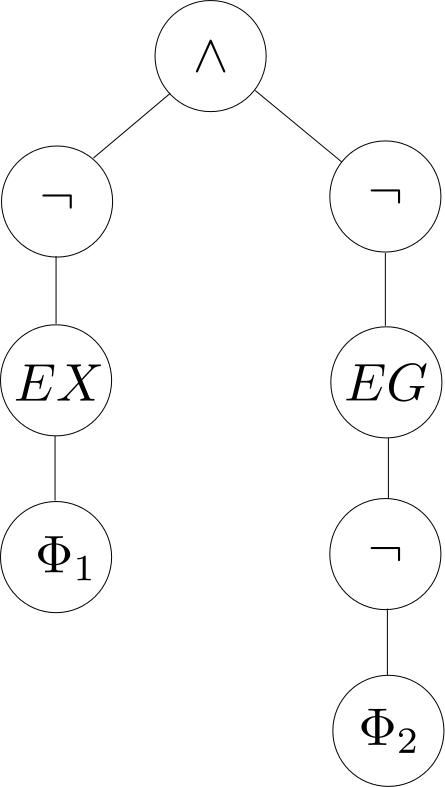
\includegraphics[scale=.4]{abstract_syntax_tree.png}
\caption{Abstract syntax tree}
\label{fig:ast}
\end{figure}

The sub-terms are defined from the atoms up:

$\Phi_1: Sat(\Phi_1)$

$EX \Phi_1: \{s \in S | Succ(s) \cap Sat(\Phi_1) \neq \emptyset\}$

$\neg (EX \Phi_1): S \setminus \{s \in S | Succ(s) \cap Sat(\Phi_1) \neq \emptyset\}$

$\Phi_2: Sat(\Phi_2)$

$\neg \Phi_2: S \setminus Sat(\Phi_2)$

$EG \neg \Phi_2: T, \text{    where } \{s \in S \setminus Sat(\Phi_2) | Succ(s) \cap T \neq \emptyset \} \supseteq T, \text{greatest } T$

$\neg (EG \neg \Phi_2): S \setminus Sat(EG \neg \Phi_2)$

$\neg (EX \Phi_1) \wedge (\neg (EG \neg \Phi_2)): Sat(\neg (EX \Phi_1)) \cap Sat(\neg (EG \neg \Phi_2))$

A sub-term whose set of states is defined recursively is the sub-term $EG \neg \Phi_2$.
The recursion equation is $\{s \in S \setminus Sat(\Phi_2) | Succ(s) \cap T \neq \emptyset \} \supseteq T$.
This equation has many solutions.
Replacing the subset operator with equal, the recursion equation can be seen as a function $f$ of $T$.
The only solutions are then fixed-points of $f$.
A fixed-point for $f$ is a value $x_0$ that makes the following equation true: $x_0 = f(x_0)$,
namely, applying the function to the value gives the value itself, "fixed" in some sense.
It can be shown that the solutions have a unique least solution and a unique greatest solution,
or since the solutions is the same as the fixed-points for the function, a least fixed-point and a greatest fixed-point.
The least fixed-point is the empty set.
The greatest fixed-point is more interesting, and is exactly equal to $EG \neg \Phi_2$.
If the equation had not been an existential-always, but an existential-until or
an existential-eventually, the interesting fixed point would be the least fixed point.

The solution to the transition system $M_1$ can be calculated recursively,
using the sets found for each sub-term:

$\Phi_1: Sat(\Phi_1): \{s_0, s_4, s_5\}$

$EX \Phi_1: \{s \in S | Succ(s) \cap Sat(\Phi_1) \neq \emptyset\}: \{s_1, s_2, s_3\}$

$\neg (EX \Phi_1): S \setminus Sat(EX \Phi_1): \{s_0, s_4, s_5\}$

$\Phi_2: Sat(\Phi_2): \{s_1, s_2, s_3\}$

$EG \neg \Phi_2: \neg \Phi_2: S \setminus Sat(\Phi_2): \{s_0, s_4, s_5\}$

$EG \neg \Phi_2: T, \text{    where } \{s \in Sat(\neg \Phi_2) | Succ(s) \cap T \neq \emptyset \} \supseteq T, \text{greatest } T: \{\}$

$\neg (EG \neg \Phi_2): S \setminus Sat(EG \neg \Phi_2): \{s_0, s_1, s_2, s_3, s_4, s_5\}$

$\neg (EX \Phi_1) \wedge (\neg (EG \neg \Phi_2)): Sat(\neg (EX \Phi_1)) \cap Sat(\neg (EG \neg \Phi_2)): \{s_0, s_4, s_5\}$

